\section{Resultados}
\label{sec:resultados}

Esta seção apresenta os resultados obtidos após a revisão final do fluxo
DSSAT--PPO. Primeiro são mostrados os resultados da calibração da produtividade
simulada contra o rendimento observado do SIDRA. Em seguida são apresentados a
avaliação do agente PPO, a comparação com políticas de referência e um exemplo de
uso operacional para uma safra recente. As tabelas foram geradas a partir dos
arquivos em \texttt{outputs/calibration\_v4\_row\_bias\_corrected/} e
\texttt{outputs/ppo\_soja\_castro\_dssat/}.

\subsection{Calibração da produtividade simulada}
\label{subsec:resultados_calibracao}

A produtividade bruta do DSSAT apresentou desvios relevantes em relação ao
rendimento médio observado no SIDRA. Por esse motivo, foi aplicada a correção
estatística descrita na metodologia. A seleção do parâmetro de regularização foi
feita no conjunto de validação, após ajuste de intercepto pelo viés médio de
validação. O valor selecionado foi $\alpha = 200$.

\begin{table}[htbp]
\centering
\caption{Desempenho da correção de produtividade DSSAT por conjunto temporal.}
\label{tab:metricas_calibracao}
\begin{tabular}{lrrrrr}
\hline
Conjunto & MAE & RMSE & MAPE & Viés & $n$ \\
         & (kg ha$^{-1}$) & (kg ha$^{-1}$) & (\%) & (kg ha$^{-1}$) & \\
\hline
Treinamento & 229,56 & 319,94 & 7,49 & 136,40 & 12 \\
Validação   & 109,06 & 138,63 & 2,82 & 0,00   & 4  \\
Teste       & 111,82 & 146,95 & 2,75 & -64,44 & 3  \\
\hline
\end{tabular}
\end{table}

No conjunto de teste, composto pelos anos de 2022, 2023 e 2024, o erro absoluto
médio foi de 111,82 kg ha$^{-1}$. O viés médio foi de -64,44 kg ha$^{-1}$,
indicando leve subestimação no teste. A Tabela~\ref{tab:calibracao_ano} mostra
os valores por ano.

\begin{table}[htbp]
\centering
\caption{Produtividade observada e produtividade DSSAT corrigida no conjunto de teste.}
\label{tab:calibracao_ano}
\begin{tabular}{rrrrr}
\hline
Ano & Observado & DSSAT corrigido & Erro & Erro absoluto \\
    & (kg ha$^{-1}$) & (kg ha$^{-1}$) & (kg ha$^{-1}$) & (\%) \\
\hline
2022 & 3.923 & 3.902,11 & -20,89  & 0,53 \\
2023 & 4.154 & 3.910,49 & -243,51 & 5,86 \\
2024 & 3.827 & 3.898,07 & 71,07   & 1,86 \\
\hline
\end{tabular}
\end{table}

A Figura~\ref{fig:dssat_obs_pred} compara produtividade observada e prevista
após a correção. Os pontos de validação e teste ficaram próximos da linha 1:1,
com maior erro em 2023. A Figura~\ref{fig:dssat_erro_ano} mostra o erro por ano.
O ano de 2009 permaneceu como o maior desvio no conjunto de treinamento, com
superestimação de 865,42 kg ha$^{-1}$. Como esse ano pertence ao treinamento, ele
não altera a leitura do desempenho externo, mas indica que a série municipal tem
anos de difícil ajuste com as variáveis usadas.

\begin{figure}[htbp]
\centering
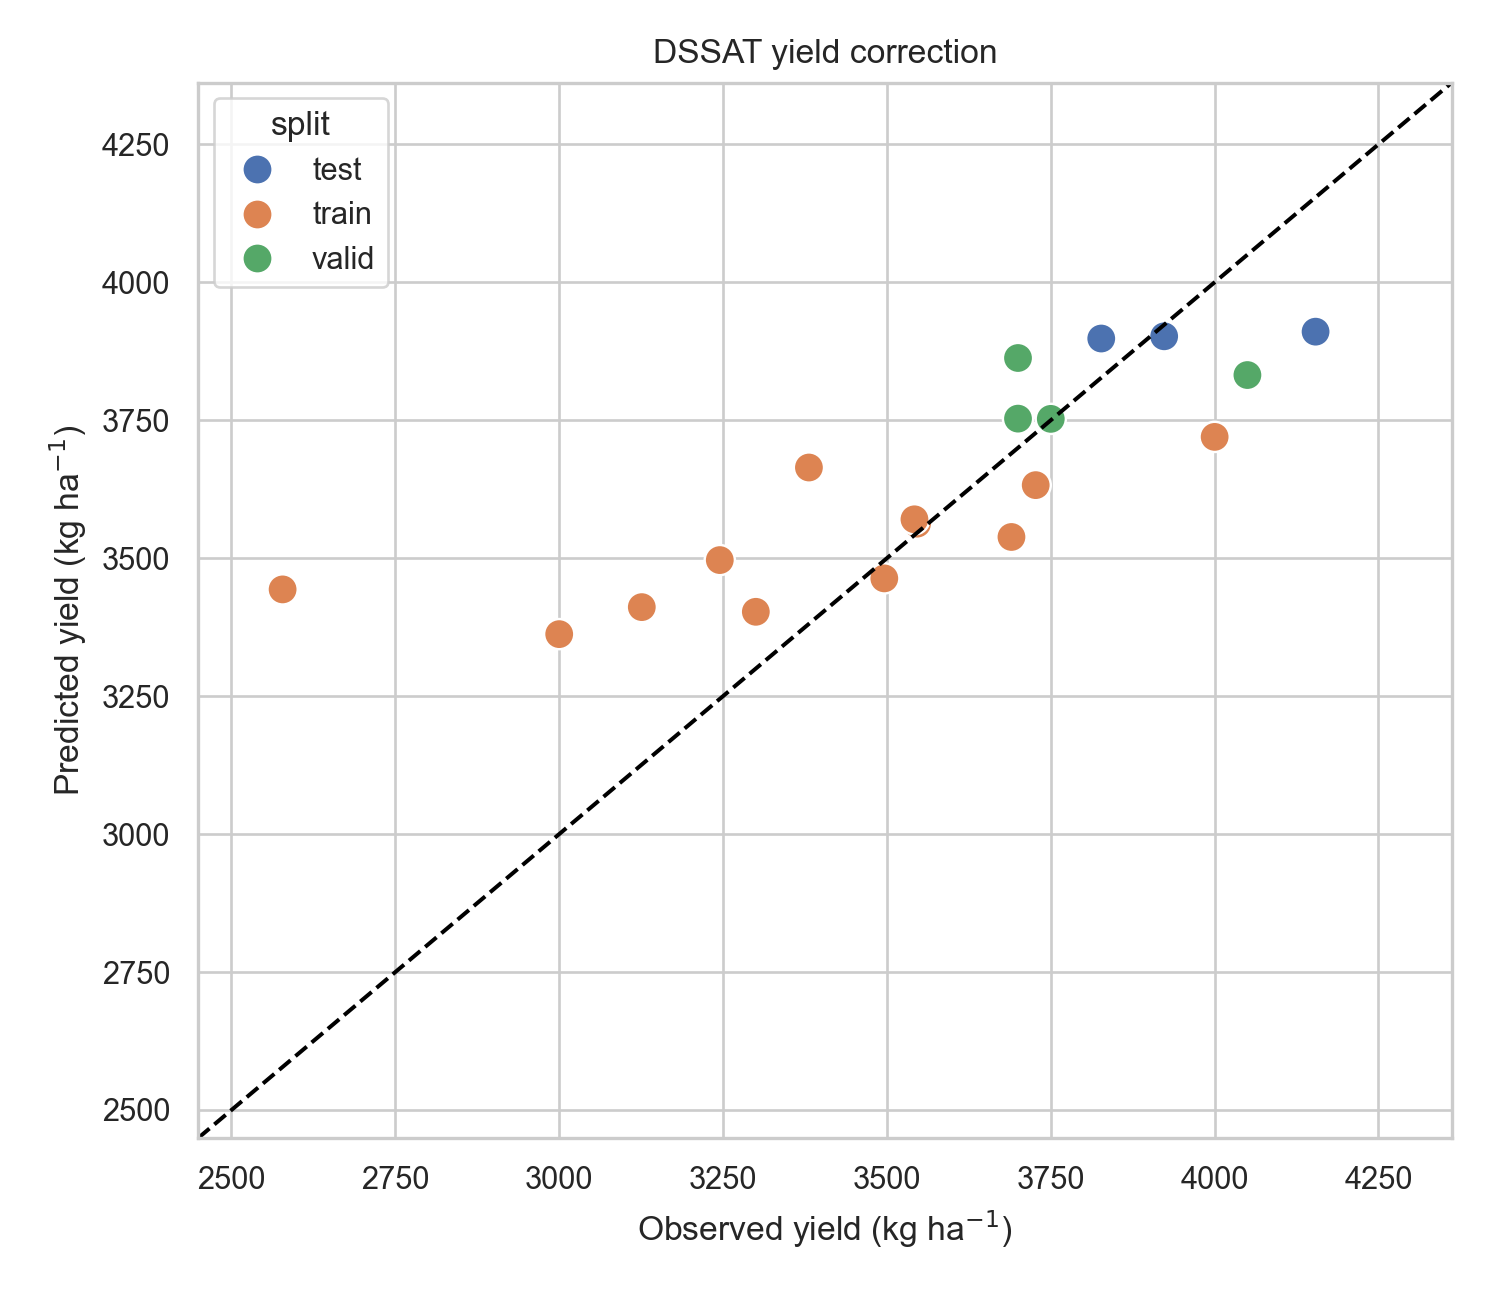
\includegraphics[width=0.82\textwidth]{dssat_rl_soybean/outputs/calibration_v4_row_bias_corrected/figures/dssat_observed_vs_corrected_yield_en.png}
\caption{Produtividade observada e produtividade estimada pelo DSSAT após correção.}
\label{fig:dssat_obs_pred}
\end{figure}

\begin{figure}[htbp]
\centering
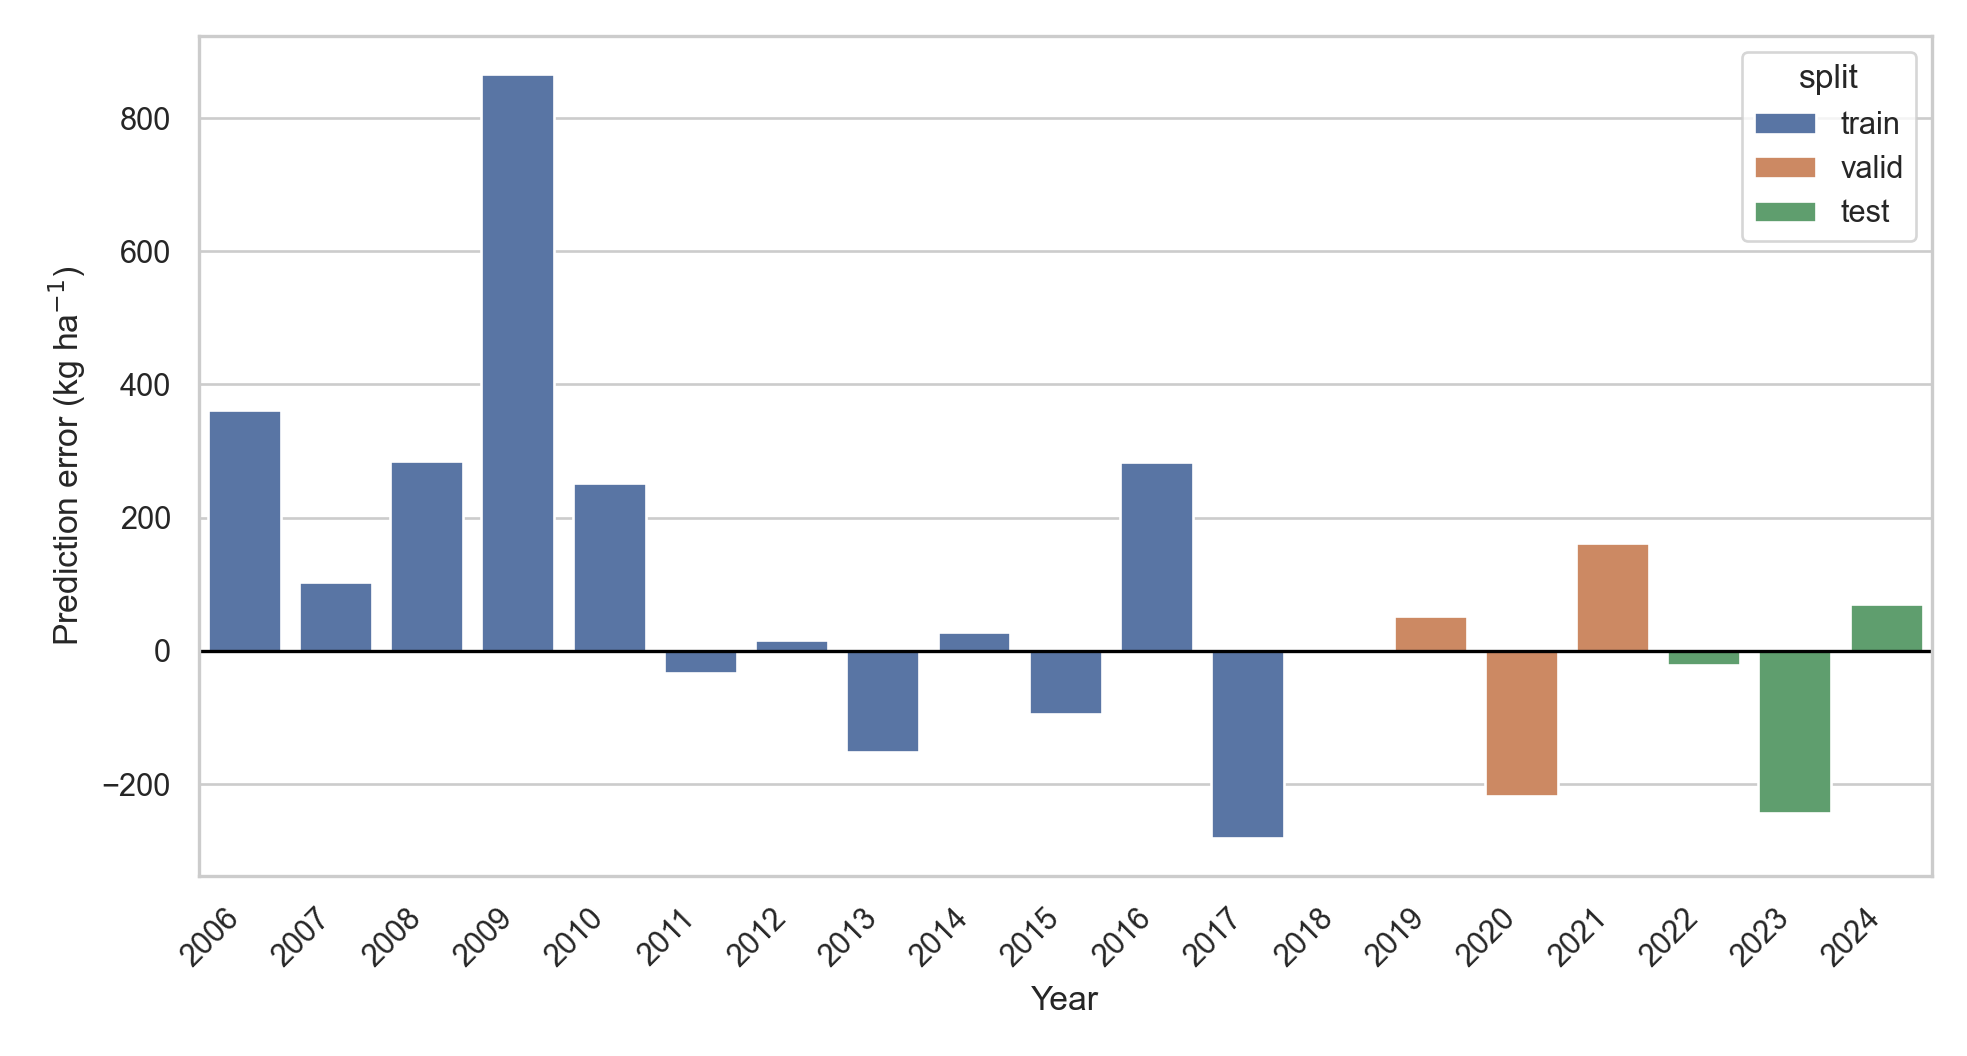
\includegraphics[width=0.90\textwidth]{dssat_rl_soybean/outputs/calibration_v4_row_bias_corrected/figures/dssat_correction_error_by_year_en.png}
\caption{Erro anual da produtividade DSSAT corrigida em relação ao SIDRA.}
\label{fig:dssat_erro_ano}
\end{figure}

\subsection{Treinamento e seleção do PPO}
\label{subsec:resultados_treinamento}

O treinamento PPO foi configurado para até 500.000 etapas, com avaliação no
conjunto de validação a cada 10.000 etapas. A maior recompensa média registrada
na curva de validação ocorreu em 90.000 etapas, com recompensa média de 0,699,
produtividade média de 3.019,88 kg ha$^{-1}$ e irrigação média de 5,69 mm. A
execução foi encerrada em 170.000 etapas pelo critério de parada por validação.

\begin{table}[htbp]
\centering
\caption{Pontos selecionados da curva de validação durante o treinamento PPO.}
\label{tab:curva_validacao}
\begin{tabular}{rrrrr}
\hline
Etapas & Recompensa média & Desvio & Produtividade média & Irrigação média \\
       &                  &        & (kg ha$^{-1}$)       & (mm) \\
\hline
10.000  & 0,669 & 0,433 & 3.661,91 & 58,02 \\
50.000  & 0,683 & 0,504 & 2.944,47 & 5,25  \\
90.000  & 0,699 & 0,504 & 3.019,88 & 5,69  \\
130.000 & 0,590 & 0,507 & 2.562,08 & 5,81  \\
170.000 & 0,648 & 0,529 & 2.798,09 & 5,09  \\
\hline
\end{tabular}
\end{table}

A Figura~\ref{fig:validation_learning_curve} apresenta a curva de validação
armazenada durante o treinamento. Após a calibração final do DSSAT, o modelo PPO
salvo foi reavaliado com o corretor de produtividade atualizado. Por isso, as
tabelas das próximas subseções representam a avaliação final do agente na versão
calibrada do ambiente.

\begin{figure}[htbp]
\centering
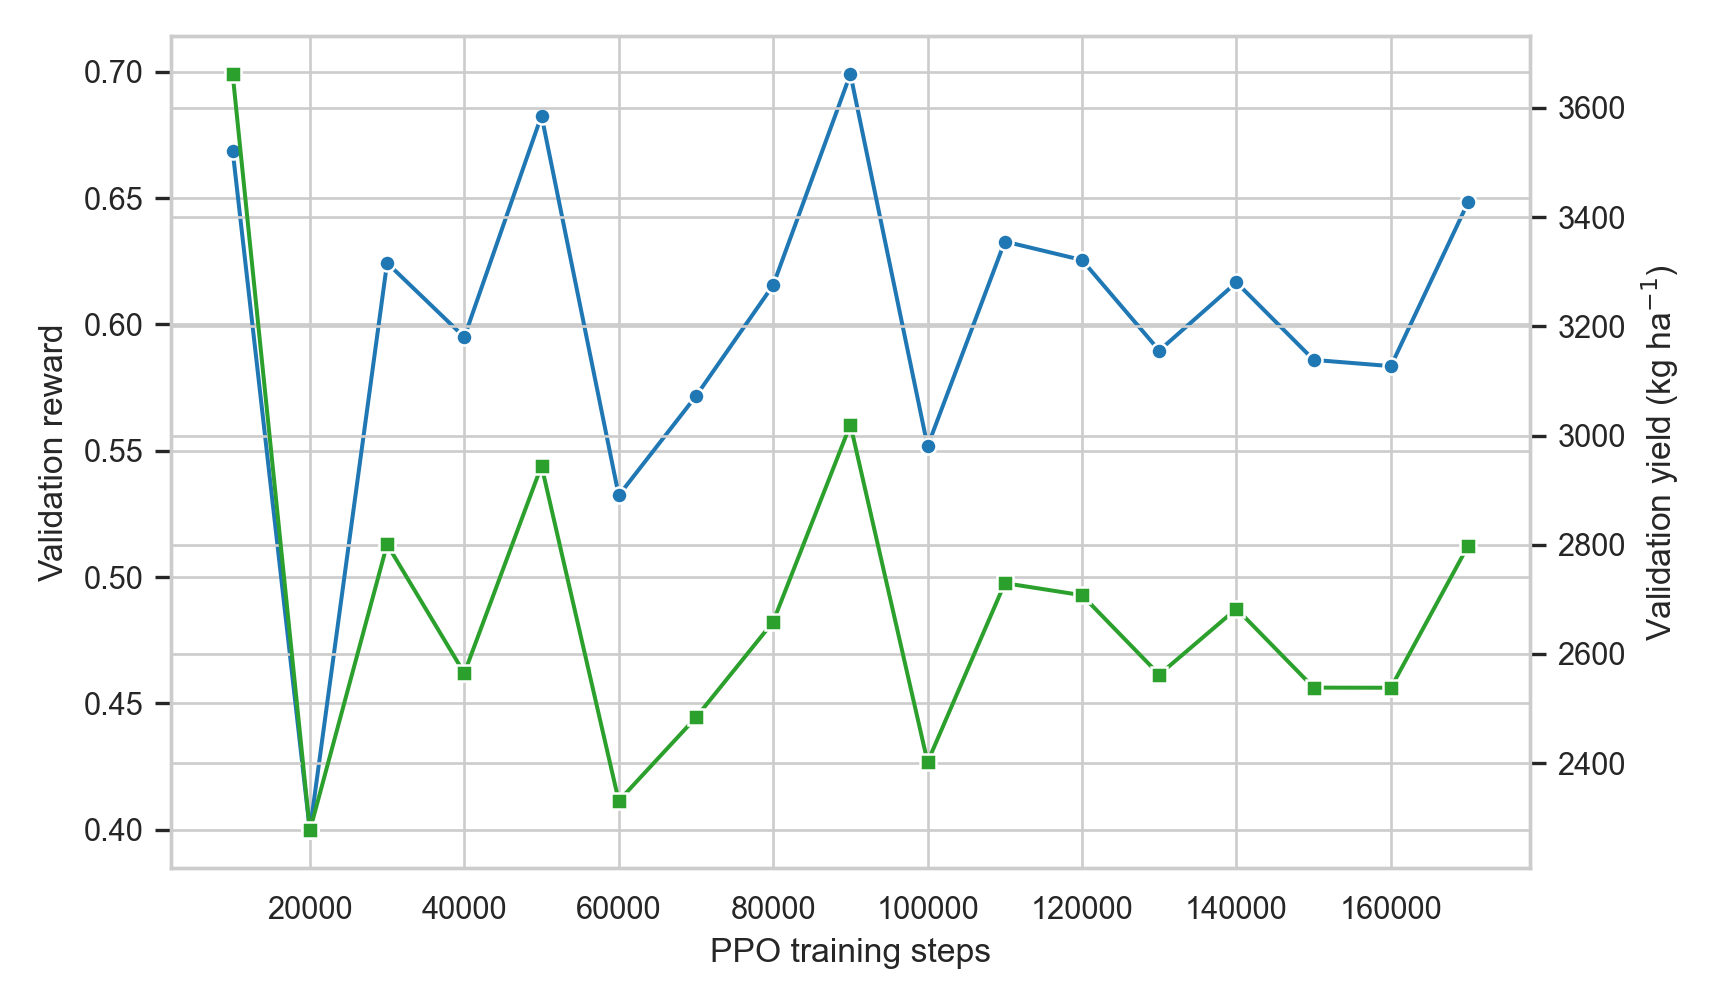
\includegraphics[width=0.86\textwidth]{dssat_rl_soybean/outputs/ppo_soja_castro_dssat/figures/validation_learning_curve_en.png}
\caption{Curva de validação registrada durante o treinamento PPO.}
\label{fig:validation_learning_curve}
\end{figure}

\subsection{Avaliação final da política PPO}
\label{subsec:avaliacao_ppo_final}

A política PPO salva foi avaliada novamente com o DSSAT calibrado. Em validação,
a produtividade média foi de 3.808,07 kg ha$^{-1}$, com erro absoluto médio de
117,72 kg ha$^{-1}$. No teste, considerando apenas anos com rendimento observado
no SIDRA, o erro absoluto médio foi de 112,77 kg ha$^{-1}$ e o viés foi de
-39,75 kg ha$^{-1}$. O ano de 2025 foi mantido na simulação climática, mas não
entrou no cálculo de erro observado por não haver rendimento SIDRA disponível na
base usada.

\begin{table}[htbp]
\centering
\caption{Resumo da avaliação final da política PPO com DSSAT calibrado.}
\label{tab:ppo_resumo_final}
\begin{tabular}{lrrrrrr}
\hline
Conjunto & Recompensa & Produtividade & Irrigação & MAE & MAPE & $n$ \\
         & média & média & média & & & \\
         &       & (kg ha$^{-1}$) & (mm) & (kg ha$^{-1}$) & (\%) & \\
\hline
Validação & 0,907 & 3.808,07 & 0,00 & 117,72 & 3,05 & 4 \\
Teste     & 0,940 & 3.950,51 & 0,50 & 112,77 & 2,80 & 4 \\
\hline
\end{tabular}
\end{table}

\begin{table}[htbp]
\centering
\caption{Resultados anuais da política PPO no conjunto de validação.}
\label{tab:ppo_validacao}
\begin{tabular}{rrrrrrr}
\hline
Ano & Plantio & Produtividade & Observado & Erro & Irrigação & Chuva \\
    &         & (kg ha$^{-1}$) & (kg ha$^{-1}$) & (kg ha$^{-1}$) & (mm) & (mm) \\
\hline
2018 & 29/09 & 3.763,59 & 3.750 & 13,59   & 0 & 738 \\
2019 & 02/10 & 3.773,91 & 3.700 & 73,91   & 0 & 573 \\
2020 & 30/09 & 3.830,71 & 4.050 & -219,29 & 0 & 667 \\
2021 & 27/09 & 3.864,08 & 3.700 & 164,08  & 0 & 641 \\
\hline
\end{tabular}
\end{table}

\begin{table}[htbp]
\centering
\caption{Resultados anuais da política PPO no conjunto de teste.}
\label{tab:ppo_teste}
\begin{tabular}{rrrrrrr}
\hline
Ano & Plantio & Produtividade & Observado & Erro & Irrigação & Chuva \\
    &         & (kg ha$^{-1}$) & (kg ha$^{-1}$) & (kg ha$^{-1}$) & (mm) & (mm) \\
\hline
2022 & 27/09 & 3.904,62 & 3.923 & -18,38  & 0 & 714 \\
2023 & 29/09 & 3.943,61 & 4.154 & -210,39 & 0 & 844 \\
2024 & 02/10 & 3.936,53 & 3.827 & 109,53  & 2 & 647 \\
2025 & 27/09 & 4.017,29 & --    & --      & 0 & 623 \\
\hline
\end{tabular}
\end{table}

As decisões do agente se concentraram no início da janela de plantio, entre 27
de setembro e 2 de outubro. O gatilho de déficit hídrico ficou em 90 mm em todos
os anos avaliados, e a lâmina por evento foi de 2 mm. Na avaliação final, essa
combinação levou a manejo quase sequeiro: apenas 2024 recebeu irrigação, com 2
mm aplicados em um evento. Esse comportamento é coerente com a função de
recompensa, que penaliza a água aplicada e, ao mesmo tempo, usa a produtividade
corrigida como retorno principal.

A Figura~\ref{fig:ppo_obs_pred} mostra a comparação entre produtividade observada
e prevista pela política PPO. A Figura~\ref{fig:ppo_yield_dist} mostra a
distribuição das produtividades simuladas e os pontos observados.

\begin{figure}[htbp]
\centering
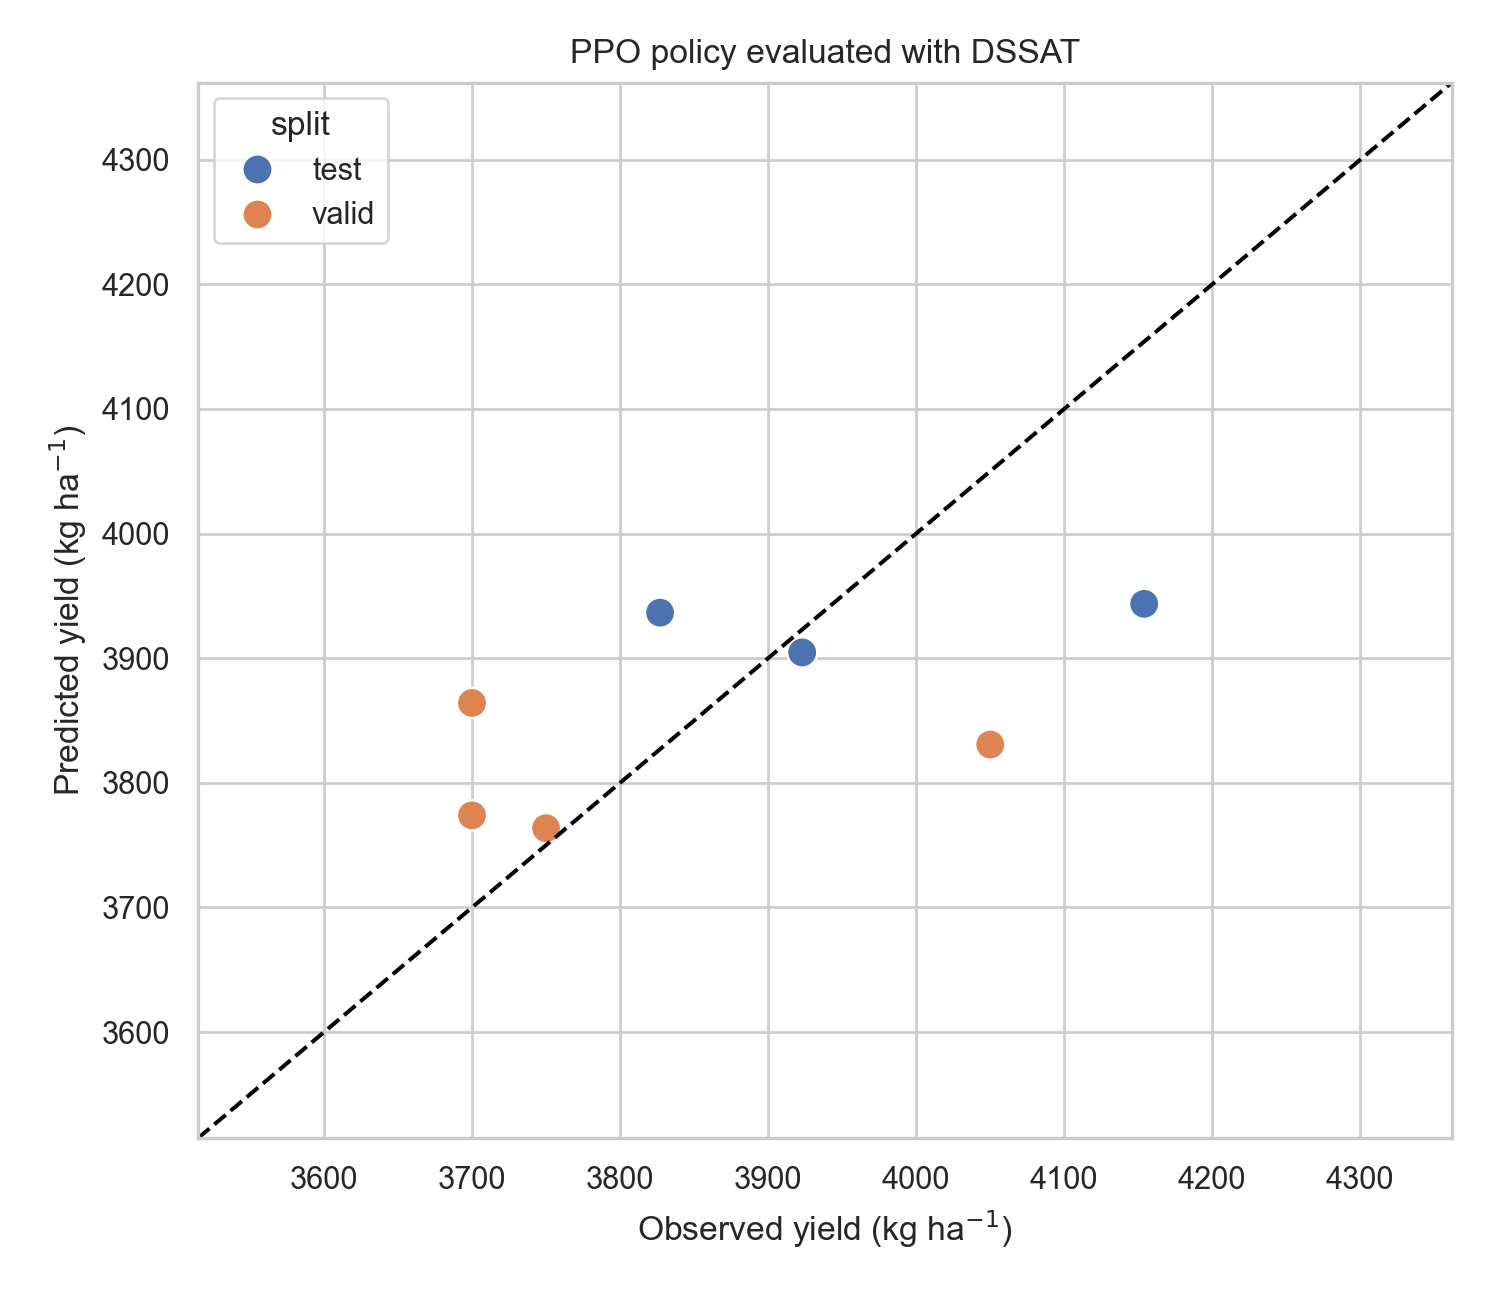
\includegraphics[width=0.82\textwidth]{dssat_rl_soybean/outputs/ppo_soja_castro_dssat/figures/ppo_observed_vs_predicted_yield_en.png}
\caption{Produtividade observada e produtividade simulada pela política PPO.}
\label{fig:ppo_obs_pred}
\end{figure}

\begin{figure}[htbp]
\centering
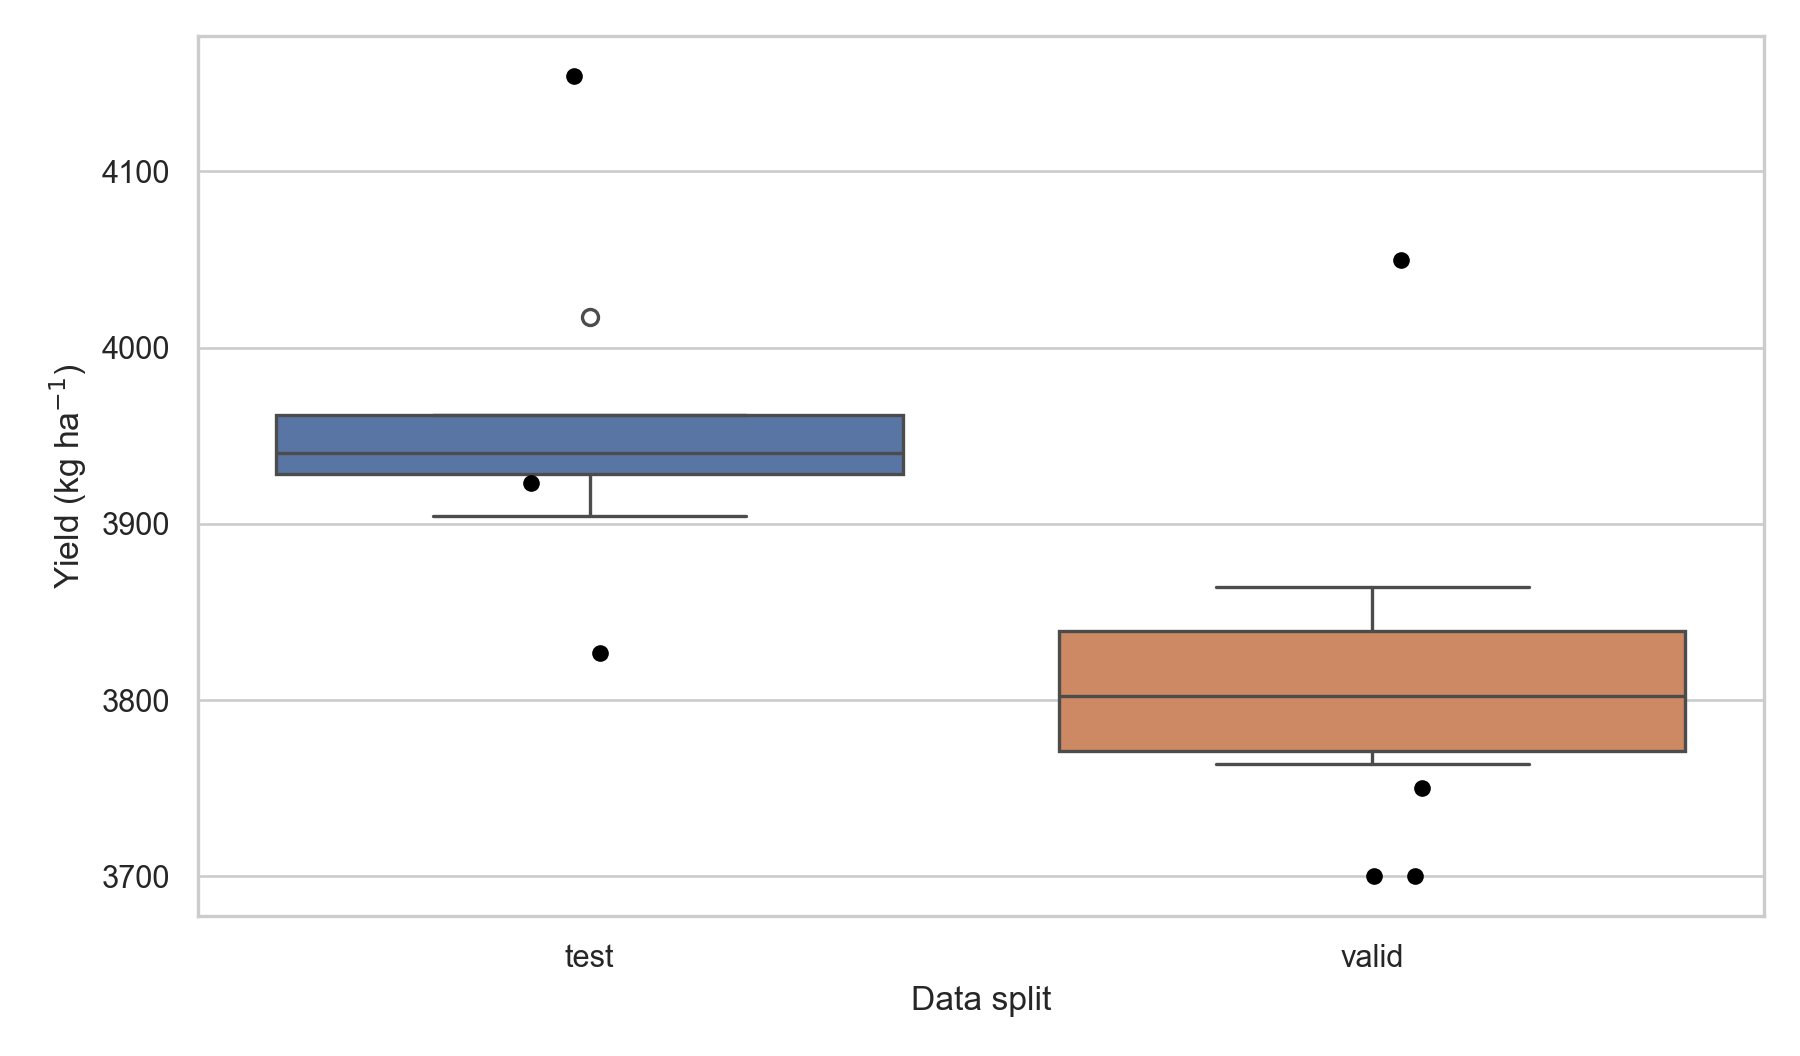
\includegraphics[width=0.82\textwidth]{dssat_rl_soybean/outputs/ppo_soja_castro_dssat/figures/ppo_yield_distribution_en.png}
\caption{Distribuição da produtividade simulada pela política PPO e valores observados.}
\label{fig:ppo_yield_dist}
\end{figure}

\subsection{Comparação com políticas de referência}
\label{subsec:comparacao_politicas}

A política PPO foi comparada com quatro manejos fixos: plantio em 15 de outubro
sem irrigação, plantio em 15 de outubro com irrigação moderada, plantio em 25 de
setembro com irrigação moderada e plantio em 10 de novembro com irrigação
moderada. As políticas irrigadas aplicaram água somente quando a regra de déficit
hídrico acionou eventos dentro da safra.

\begin{table}[htbp]
\centering
\caption{Comparação entre PPO e políticas de referência na validação.}
\label{tab:comparacao_validacao}
\begin{tabular}{lrrr}
\hline
Política & Recompensa média & Produtividade média & Irrigação média \\
         &                  & (kg ha$^{-1}$)      & (mm) \\
\hline
PPO & 0,907 & 3.808,07 & 0,00 \\
Sequeiro 15/out & 0,906 & 3.805,81 & 0,00 \\
25/set irrigado & 0,871 & 3.800,02 & 22,50 \\
10/nov irrigado & 0,871 & 3.801,42 & 22,50 \\
15/out irrigado & 0,864 & 3.796,99 & 27,00 \\
\hline
\end{tabular}
\end{table}

\begin{table}[htbp]
\centering
\caption{Comparação entre PPO e políticas de referência no teste.}
\label{tab:comparacao_teste}
\begin{tabular}{lrrr}
\hline
Política & Recompensa média & Produtividade média & Irrigação média \\
         &                  & (kg ha$^{-1}$)      & (mm) \\
\hline
PPO & 0,940 & 3.950,51 & 0,50 \\
Sequeiro 15/out & 0,939 & 3.945,76 & 0,00 \\
25/set irrigado & 0,919 & 3.944,88 & 13,50 \\
15/out irrigado & 0,881 & 3.926,69 & 36,00 \\
10/nov irrigado & 0,861 & 3.926,78 & 49,50 \\
\hline
\end{tabular}
\end{table}

Na validação, o PPO apresentou recompensa média de 0,907, valor muito próximo da
política sequeira de 15 de outubro, que atingiu 0,906. A produtividade média do
PPO foi 2,26 kg ha$^{-1}$ maior. No teste, o PPO também ficou ligeiramente acima
do sequeiro em recompensa e produtividade média. A diferença foi pequena:
3.950,51 kg ha$^{-1}$ no PPO contra 3.945,76 kg ha$^{-1}$ no sequeiro. O agente
aplicou 0,5 mm em média no teste, devido ao evento de 2 mm em 2024.

As políticas irrigadas fixas apresentaram recompensas menores, mesmo com
produtividades próximas, porque o ganho em rendimento não compensou a penalização
da água na função de recompensa. Esse resultado indica que, sob a parametrização
atual e após a correção da produtividade, o ambiente favoreceu manejos de baixa
irrigação para os anos avaliados.

\begin{figure}[htbp]
\centering
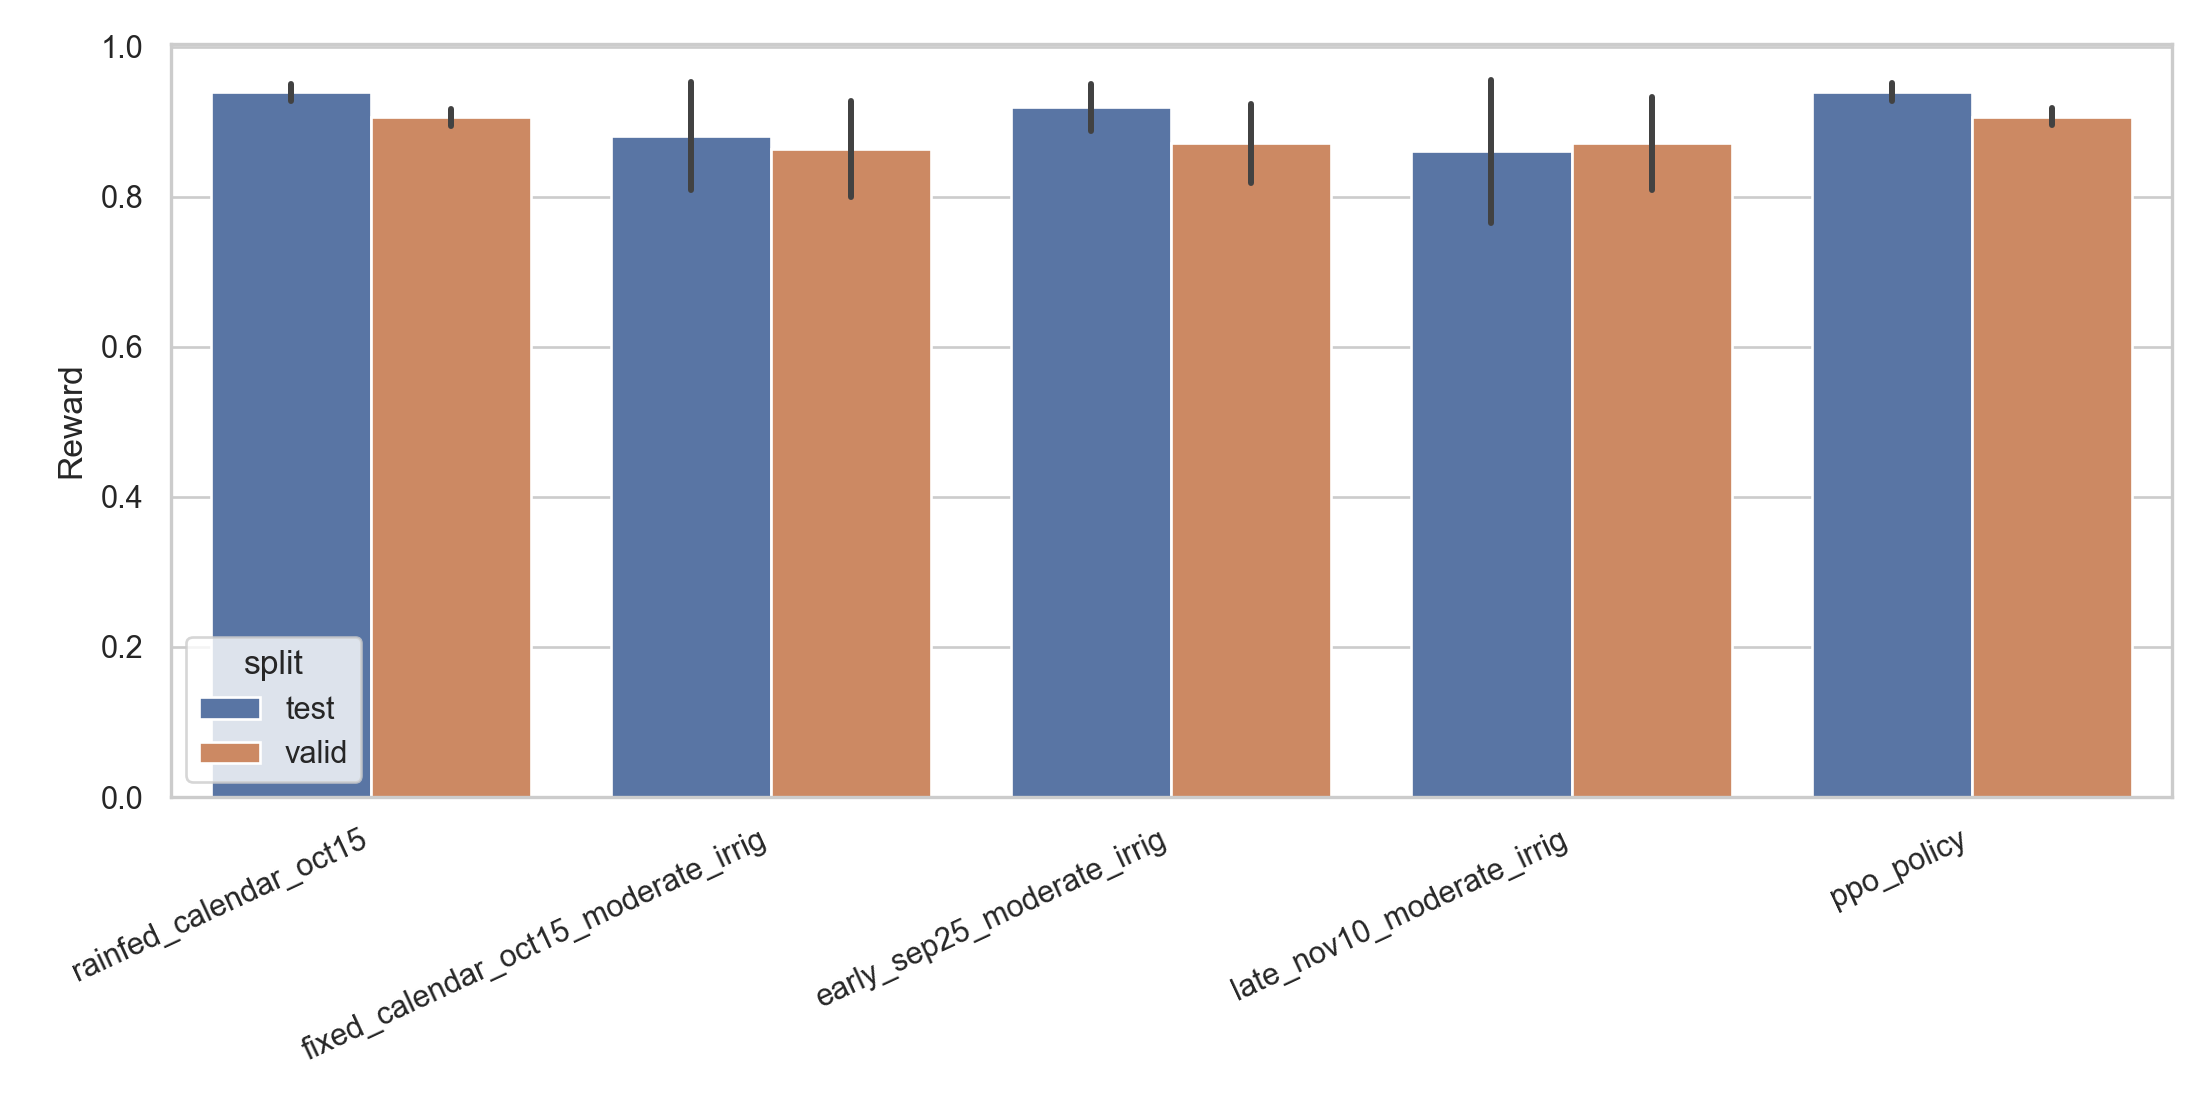
\includegraphics[width=0.86\textwidth]{dssat_rl_soybean/outputs/ppo_soja_castro_dssat/figures/ppo_vs_baselines_reward_en.png}
\caption{Recompensa da política PPO e das políticas de referência.}
\label{fig:ppo_vs_baselines_reward}
\end{figure}

\begin{figure}[htbp]
\centering
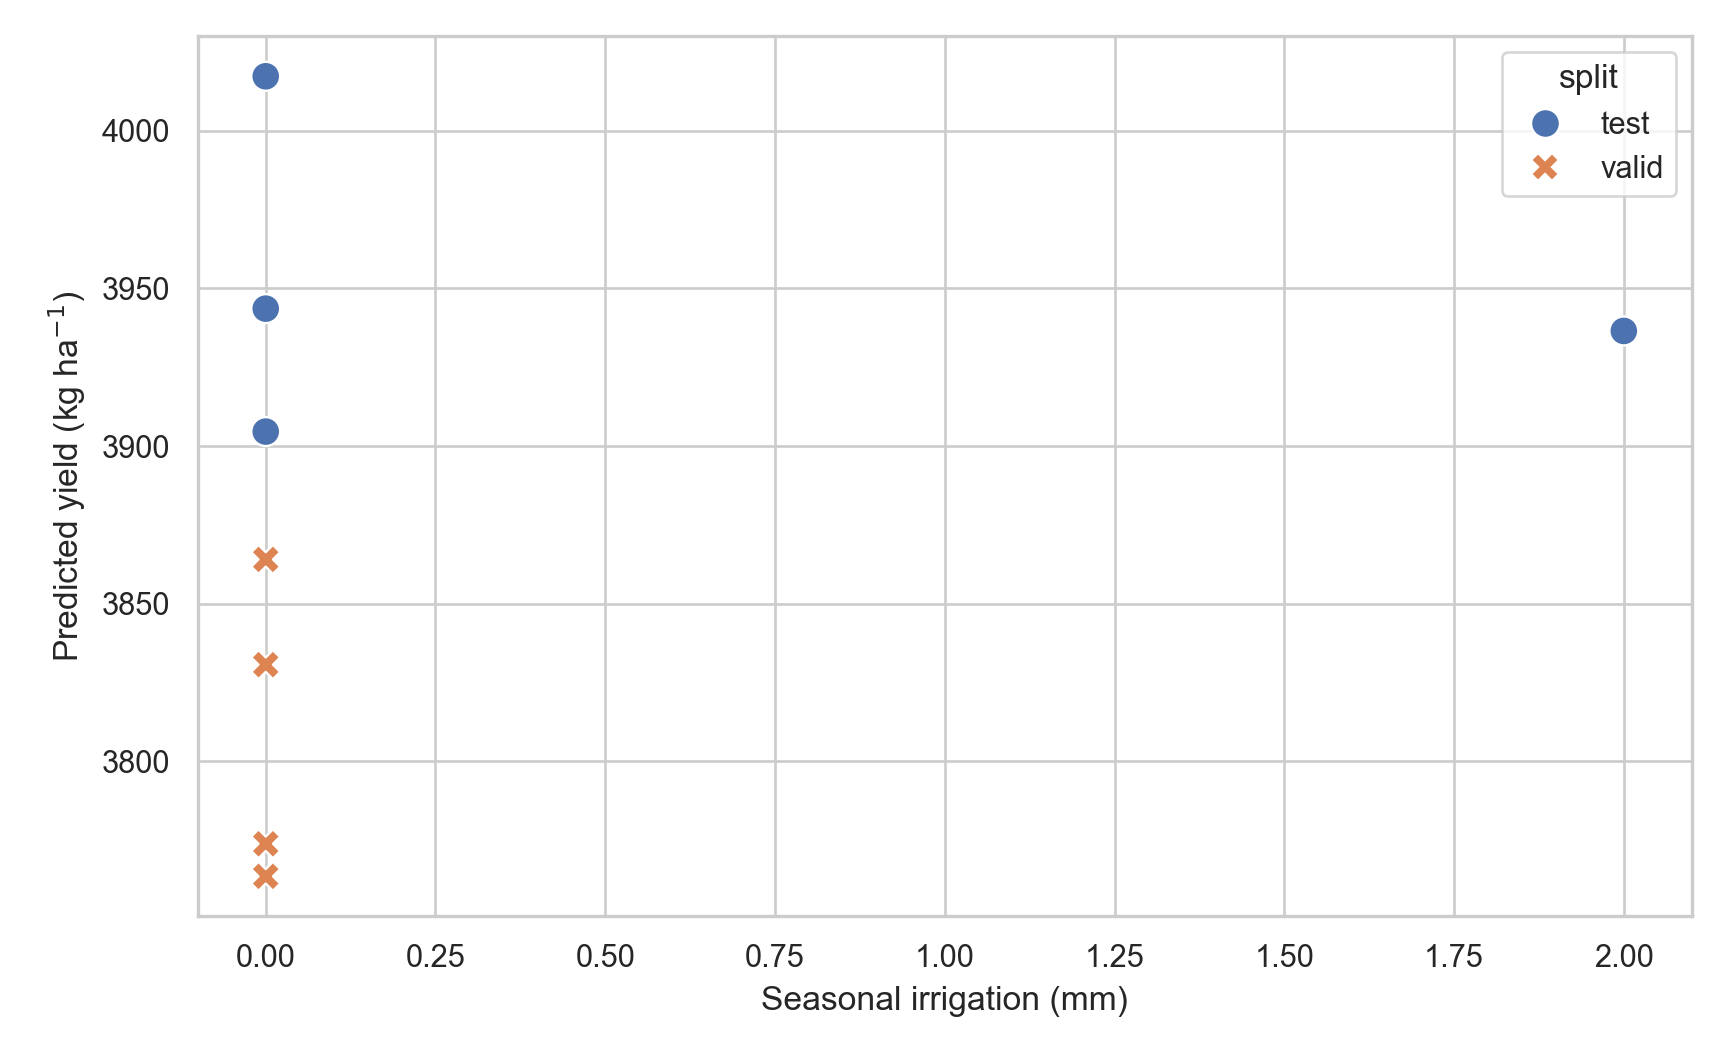
\includegraphics[width=0.82\textwidth]{dssat_rl_soybean/outputs/ppo_soja_castro_dssat/figures/ppo_yield_water_tradeoff_en.png}
\caption{Relação entre produtividade simulada e irrigação sazonal.}
\label{fig:ppo_yield_water_tradeoff}
\end{figure}

\subsection{Exemplo de uso operacional}
\label{subsec:exemplo_uso}

Para exemplificar o uso do agente em modo operacional, foi executada uma
recomendação para a safra de 2025, usando a série meteorológica disponível na
base. O modelo indicou plantio em 27 de setembro de 2025, gatilho de déficit
hídrico de 90 mm, lâmina de 2 mm por evento e limite sazonal de 36,26 mm. A
simulação resultante não acionou irrigação, pois a regra de déficit não atingiu
o limite definido pelo agente. O resultado esperado foi produtividade de
4.017,29 kg ha$^{-1}$, precipitação acumulada de 623 mm e recompensa de 0,956.

\begin{table}[htbp]
\centering
\caption{Exemplo de recomendação operacional para a safra de 2025.}
\label{tab:exemplo_operacional}
\begin{tabular}{lr}
\hline
Item & Valor \\
\hline
Data de plantio recomendada & 27/09/2025 \\
Gatilho de déficit hídrico & 90 mm \\
Lâmina por evento & 2 mm \\
Limite sazonal de irrigação & 36,26 mm \\
Irrigação simulada & 0 mm \\
Chuva na janela simulada & 623 mm \\
Produtividade simulada & 4.017,29 kg ha$^{-1}$ \\
Recompensa & 0,956 \\
\hline
\end{tabular}
\end{table}

Esse exemplo mostra como o agente pode ser usado para transformar uma safra
meteorológica em uma decisão de manejo. Em uso de campo, a recomendação deve ser
gerada com previsão meteorológica atualizada, solo calibrado e cultivar validada
para a área. A saída do agente deve ser interpretada como apoio à decisão, pois
o manejo real ainda depende de disponibilidade de máquinas, umidade operacional
do solo, sanidade da lavoura e restrições de água.

\subsection{Síntese dos resultados}
\label{subsec:sintese_resultados}

A correção estatística reduziu o erro da produtividade simulada no teste para
111,82 kg ha$^{-1}$, com MAPE de 2,75\%. Após essa etapa, a avaliação final da
política PPO apresentou MAE de 112,77 kg ha$^{-1}$ nos anos de teste com
observação disponível. A política aprendida concentrou o plantio no fim de
setembro e início de outubro e usou pouca irrigação. A comparação com políticas
fixas mostrou que o PPO ficou muito próximo do sequeiro em recompensa, com leve
ganho de produtividade média no teste.

Os resultados indicam que o principal ganho do fluxo revisado foi a capacidade de
alinhar a produtividade simulada ao rendimento municipal observado. A etapa de
calibração tornou a avaliação do agente mais compatível com os dados reais de
Castro. Para avanços futuros, o ponto mais importante é substituir o solo padrão
por um perfil local calibrado e repetir o treinamento PPO com a versão final do
ambiente, mantendo a mesma separação temporal usada nesta análise.
